\documentclass[11pt]{article}
\usepackage{amsmath} % AMS Math Package
\usepackage{amsthm} % Theorem Formatting
\usepackage{amssymb} % Math symbols such as \mathbb
\usepackage{hyperref}
    \hypersetup{colorlinks=true,citecolor=blue,urlcolor =black,linkbordercolor={1 0 0}}
\usepackage{graphicx}
\usepackage{caption}
%\usepackage{filecontents}
\usepackage{subcaption}% Allows for eps images
\usepackage[table,xcdraw]{xcolor}
\usepackage{tikz}
\usepackage{cite}
\usepackage{siunitx}
\usepackage{tabularx} % Allows for table with custom column width
\usepackage{lipsum}
\usepackage{parskip}
\usepackage{booktabs}
%\usepackage{mathtools}
\usepackage[letterpaper, total={6.5in, 9in}]{geometry} % see geometry.pdf on how to lay out the page. There's lots.
\usepackage [english]{babel}
\usepackage [autostyle, english = american]{csquotes}
\usepackage{siunitx}
\usepackage{float}
\usepackage{array}
\usepackage{paralist}
\usepackage{ragged2e}
\usepackage{caption}
\usepackage{graphicx}
\usepackage{lipsum}
\usepackage{url}
\usepackage{hyperref}
\usepackage{wrapfig}
\usepackage{setspace} % you can control the spacing here
\onehalfspacing
\setlength\parindent{24pt}
\MakeOuterQuote{"} % or letter or a5paper or ... etc
\usepackage{multicol} %allows you to make multiple columned items
\usepackage{verbatim}
\usepackage{xcolor}

\title{}
\author{}
\date{} % delete this line to display the current date

%%% BEGIN DOCUMENT
\begin{document}

\begin{titlepage}
\centering
\vspace*{0mm}
\Large{Directional Clustering -  Design Document}
\vspace{30mm}

\begin{figure}[H]
\centering

\includegraphics[scale=0.2]{pton (1).png}
\end{figure}
\vspace{30mm}
\Large{Isabel Moreira de Oliveira, Hui Yuan, Thuy Vy Luu, Alexandros Papamatthaiou, Rafael Pastrana}\\

\vspace{8mm}
\large{Final Project  \\ APC524: Software Engineering for Scientific Computing \\ }
\large{Gabe Perez-Giz}\\
\large{Princeton University \\Fall 2020\\}

\end{titlepage}

% Document Skeleton

\section{Introduction}

\subsection{Motivation}

Principal stress fields are relevant to the design of volume-minimizing surface structures as they suggest optimal directions for material alignment. This implies that by following these directions, less material would be used to achieve a target level of structural performance. An example of applicability in concrete shell structures is to add steel reinforcement in the direction of tensile principal stresses so that the total amount of reinforcement needed is minimal.

Principal stress fields are ubiquitously computed by off-the-shelf finite element analysis (FEA) software and are represented as a cloud of vectors (i.e. a vector field). However, as principal stress fields are heterogeneous and form continuous curvilinear trajectories, it is actually difficult, for fabrication reasons, to place material (the reinforcement bars, beams, or other elements) in a way that exactly match the field directions (3D printing is an exception though). Therefore, extreme directional fidelity is cumbersome, and it is probably one of the reasons why we actually keep on building with crude orthogonal grids everywhere (take a look at the room around you, for example).

In this work, we question the heterogeneity of a principal stress field and inquire on how much we can simplify it so that we can maximize the feasibility of fabrication, while compromising as little as possible in structural performance. In short, what we want is to find the lowest possible amount of different vectors that encode the maximum amount of directional information about a principal stress field. We leverage a variety of clustering methods to this end.


\subsection{Scientific background}

\subsubsection{Principal stress directions}

In a material continuum subjected to in-plane external forces, principal stress directions correspond to the two orthogonal vectors that maximize normal stresses and nullify shear. Given a reference coordinate system $XY$ and a state of stress described by two normal stresses $\sigma_x, \sigma_y$ and one shear stress $\tau_{xy}$, the angle (also called "principal angle") needed to rotate it such that state of normal stress is maximized is defined by:

\begin{equation}
    \tan2\theta_{p} = \frac{2\tau_{xy}}{\sigma_x - \sigma_y}
\end{equation}

The rotated reference system $XY$ corresponds to the two principal stress directions. Similarly, the magnitude of the principal stresses $\sigma_1, \sigma_2$ is described by:

\begin{equation}
    \sigma_{1, 2} = \frac{\sigma_x + \sigma_y}{2} \pm \sqrt{(\sigma_x + \sigma_y)^2 + \tau_{xy}^2}
\end{equation}

\subsubsection{Vector field clustering}

Drawing parallels from image quantization, the directional simplification of a principal stress field is formulated as a clustering problem. The aim is to find the smallest set of vectors in $\mathbb{R}^3$ that best summarizes a principal stress field $\mathbf{F}$ within a certain distortion budget. Clustering takes place as a distance-driven process, where every principal stress vector $\mathbf{v} \in \mathbf{F}$ is assigned to the single cluster $\mathcal{C}$ whose centroid $\mathbf{c}$ is the closest.

For KMeans, the clustering process contemplates five stages: initialization, association, centroid recalculation, and termination. Let $k$ be a target number of clusters to form, $\mathbf{F}$ the principal stress field to cluster, $\mathbf{W} \in \mathbb{R}^{k \times 3}$ a matrix that stores all cluster centroids $\mathbf{c}$, and $e$ the number of epochs to run the algorithm for. To start with a reasonable estimate for  $\mathbf{W}_0$, the algorithm starts by selecting $k$ vectors $\mathbf{v}$ from $\mathbf{F}$. A loss function is introduced to evaluate the quality of the clustering with the intention to be minimized, and is defined by: 

\begin{equation}
    \mathcal{L}^{k} = \frac{1}{|\textbf{F}|} \sum^{n}_{i=1} \min_j (\mathbf{v}_{i} - \mathbf{c}_{j})^{2}
\end{equation}

Please refer to \href{https://drive.google.com/file/d/1gH3feZg796jewtrcDC3sTIwqYr9KsBPV/view}{{\textcolor{blue}{this report}}} for more details on the clustering scientific underpinnings.

\begin{comment}
WIP

Writing equations in Latex form here for further use 

\begin{equation}
    \mathcal{L}^{k} = \frac{1}{|\textbf{a}|} \sum^{n}_{i=1} min (\alpha_{i} - \theta_{j})^{2}_{j} 
\end{equation}

\begin{equation}
    w_{t+1}[j] = \frac{1}{|\textbf{g}|} \sum_{g} \textbf{a}[\textbf{g}]
\end{equation}

\begin{equation}
    \Delta^{k} = |\frac{\mathcal{L}^{k}_{t}-\mathcal{L}^{k}_{t+1}}{\mathcal{L}^{k}_{t+1}}|
\end{equation}

\begin{equation}
    \text{tan}^{-1} \text{ } 2(y,x) = \begin{cases}
    \text{tan}^{-1}(\frac{y}{x}), & \text{if } x > 0
    \\
    \text{tan}^{-1}(\frac{y}{x}) + \pi, & \text{if } x > 0, \text{ } y \geq 0
    \\
    \text{tan}^{-1}(\frac{y}{x}) - \pi, & \text{if } x < 0, \text{ } y < 0
    \\
    +\frac{\pi}{2}, & \text{if } x = 0, \text{ } y > 0
    \\
    -\frac{\pi}{2}, & \text{if } x = 0, \text{ } y < 0
    \\
    \text{undefined}, & \text{if } x = 0, \text{ } y = 0

    \end{cases}
\end{equation}


\textbf{Vector field clustering}
WIP
\end{comment}

\section{Software Architecture}

\subsection{Design Features}
Our goal is to start a modular open-source library to study the directional simplification of principal stress fields on polygonal meshes in $\mathbb{R}^3$ using a number of different clustering algorithms. To this end, we expect our library to have the following functionality: 

\begin{itemize}
    \item Independence from proprietary CAD software.
    \item A wrapper around an existing FEA library to simplify the structural analysis of meshes and to facilitate the subsequent generation of principal stress fields.
    \item An in-built library of 4 clustering vector algorithms such as KMeans, Variational KMeans, and 2 more to be defined.
    \item A 3d viewer capable to display meshes, FEA information, and the results created by the clustering algorithms. We believe it is critical to provide users with visual feedback during all steps of the process.
\end{itemize}

\subsection{Current state of affairs}
We depart from Rafael's previous research work which is stored in \href{http://www.github.com/arpastrana/directional_clustering}{\textcolor{blue}{this repository}}. The existing code consists of a small number of modules, functions, and scripts that require extensive refactoring in order to become a public library. At this point, the two most relevant functions are a custom implementation of the KMeans clustering algorithm that uses cosine distance as the basis for vector association and a simple 2D plotter for visualization. Technically, the current approach only handles polygonal meshes in $\mathbb{R}^2$ and relies on desktop FEA software \href{http://www.karamba3d.com/}{\textcolor{blue}{Karamba3d}} to extract principal stress fields. The work proposed here should overcome this limitations by proposing a unified and streamlined workflow.

\subsection{External dependencies}
We will continue to rely significantly on the \href{http://www.compas.dev}{\textcolor{blue}{ COMPAS }} framework as backend to handle the creation and manipulation of polygonal meshes and other geometric entities, such as circles, lines, and points. \href{http://www.numpy.org}{\textcolor{blue}{Numpy}} will be used as the basis for all the clustering algorithms. We currently have listed \href{https://scikit-learn.org/stable/index.html}{\textcolor{blue}{Scikit-learn}} as a dependency, but we aim to stop using the latter as we are relying only on one of its methods. Lastly, we are currently scouting a Python-based, open-source FEA library to interface with. Potential candidates are \href{https://www.code-aster.org/spip.php?rubrique21}{\textcolor{blue}{Code-Aster}}, \href{https://github.com/spacether/pycalculix}{\textcolor{blue}{Pycalculix}} and \href{https://openseespydoc.readthedocs.io/en/latest/}{\textcolor{blue}{OpenSeesPy}}.

\subsection{Interfaces}
We can use JSON files or COMPAS meshes.

Currently, there is one clustering algorithm implemented: KMeans. We would like to add Variational KMeans Clustering and others yet to be discussed. Therefore, we will benefit from an Abstract Base Class and a Factory Method similar to the Model and Model-Factory from Assignment 3 that returns the (pointer to a) clustering algorithm of choice.
The interface should allow for a call on only one type of clustering algorithm or multiple calls, each on a different algorithm. Then we should be able to compare each output in a Visualizer.
Perhaps the interface should also allow for runs of multiple meshes through the algorithm, this way, we could compare meshes with different boundary conditions or loads.

The Visualizer should have as input a mesh with principal stress field and plot a 2D visualization of the vectors on the respective mesh faces. We should be able to call the visualizer multiple times to create images where we can easily compare different algorithms, or different $k$ values for one given algorithm. Eventually, we might want to create GIFs for an animated visualization of the outputs. 

A current discussion is whether we should include 3D visualizers capable of showing surfaces in 3D space. If we include that option, then our visualizer should also provide room for the user to set different views of the same output - or even provide room for an interactive viewer that allows rotation/zoom-in/zoom-out of the output.

\subsection{UML Diagram}
We would like different start-points for our program. All of the enumerated options would result in \emph{"Our Mesh"}, which will hold the mesh and principal stress vectors in such a way that we can access each one separately.
\begin{enumerate}
    \item Start point:
    \begin{enumerate}
        \item Start with a COMPAS geometry. \newline
For this option, we would generate a mesh from the geometry (through \href{https://compas.dev/plugins.html}{\textcolor{blue}{COMPAS}}), pass the mesh into an FEA solver to obtain principal stress fields and get \emph{Our Mesh}.
        \item Start with FEA Solver. \newline
For this option, we would define geometry, boundary conditions, loads, and material with the given solver interface to get \emph{Our Mesh}.
        \item Start with a COMPAS mesh which already has principal stresses as face attributes and get \emph{Our Mesh}.
    \end{enumerate}
    
    \item Visualize with 3dViewer \emph{Our Mesh} and decide to continue or readjust the starting point.
    \item Continue with a clustering algorithm of our choice.
    \item Visualize the output
\end{enumerate}

These are the classes we should have in our UML (in Figure \ref{fig:uml}):

\begin{itemize}
    \item MeshGenerator
    \item Mesh (``\emph{OurMesh'')}
    \item VectorField
    \item FEASolver
    \item StructuralModel
    \item ClusteringAlgorithmFactory
    \item ClusteringAlgorithm
    \begin{itemize}
        \item ClusteringMethod
        \begin{itemize}
            \item KMeansClustering
            \item VariationalClustering
            \item OtherClusteringMethods
        \end{itemize}
    \end{itemize}
    \item 3DViewer
\end{itemize}

\begin{figure}[H]
    \centering
    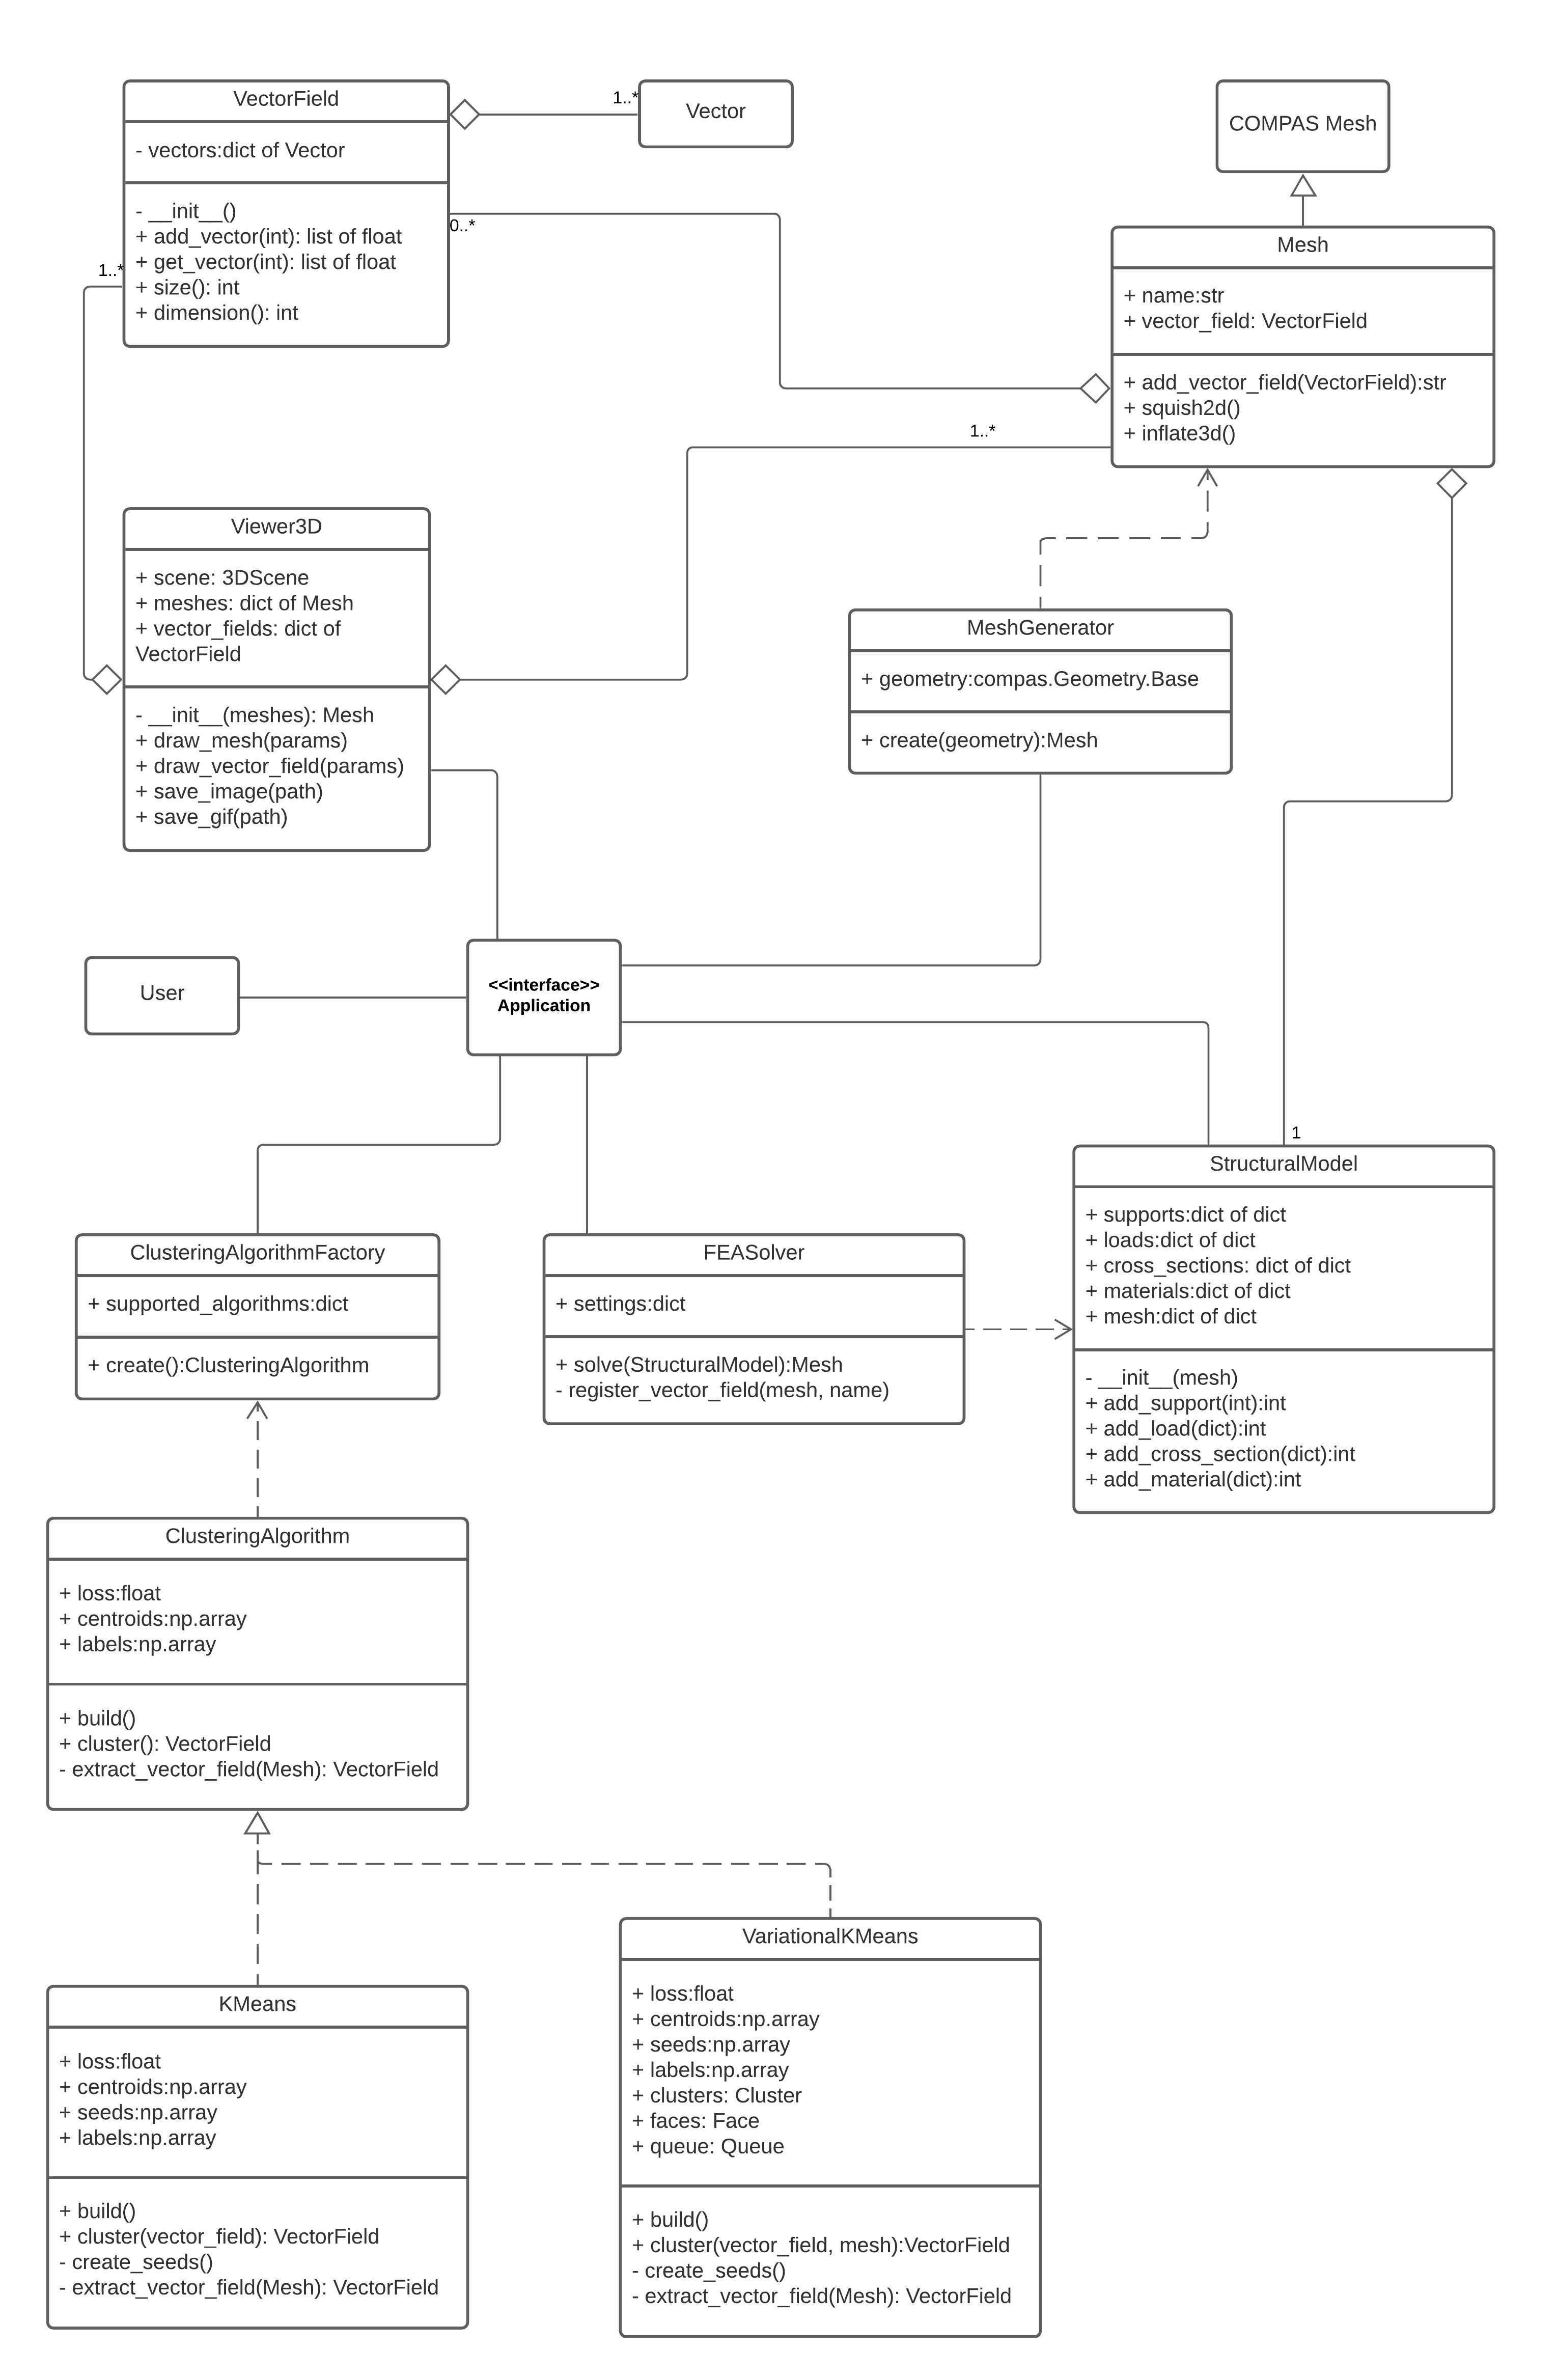
\includegraphics[scale=0.57]{UML-Clusters.jpeg}
	\caption{UML Diagram}
	\label{fig:uml}
\end{figure}
\vspace{30mm}

\section{Proposed Workflow}
We will work collaboratively on Github to make this project come to fruition. We will work on the existing repository and depart from the \href{https://github.com/arpastrana/directional_clustering/tree/apc524}{\textcolor{blue}{apc524}} branch. We will delegate tasks and make progress by simultaneously making branches. We will leverage issues and pull requests, and set up a project on Github to help us manage tasks in Kanban style. We anticipate leveraging Travis CI for continuous integration, Sphinx to build the documentation, and Pytest to run a comprehensive set of tests.

\section{Estimated Timeline}

We have \textbf{one month} to achieve alpha status, and about \textbf{two weeks} later to submit the final project. The project is planned for a total of \textbf{6 weeks}, starting next Monday October, 26th. We expect to be using most of the time in building the program architecture, doing documentation, making tests, and agreeing on interfaces. Actual coding may consequently be less of a protagonist here.

\textbf{Important deadlines:}
\begin{itemize}
    \item 01 Nov - Git + CI Setup (End of Week 1)
    \item 16 Nov - Interim review (End of Week 3)
    \item 24 Nov - Alpha version (End of Week 4)
    \item 08 Dec - Final submission (End of Week 6)
\end{itemize}

\section{Future Work}

We outline a number of directions to extend to this project further. First, enlarging the proposed library of clustering algorithms would be of genuine interest. Secondly, and if time permits, we would like to explore the creation of our minimal FEA solver that handles the structural analysis of polygonal meshes. Lastly, we envision to eventually make this package an official plugin of the \href{http://www.compas.dev}{\textcolor{blue}{COMPAS}} framework.

\end{document}
